% ------------------------------------------------------------------------
% -*-TeX-*- -*-Hard-*- Smart Wrapping
% ------------------------------------------------------------------------
\def\baselinestretch{1}

\chapter{Analysis}

\def\baselinestretch{1.66}


%%% ----------------------------------------------------------------------

In this chapter, a critical look is taken at the reviewed literature. Literature concerning the construction of learning models using machine learning was reviewed in the previous chapter, as well as literature concerning different approaches to solving the counting problem. The reviewed methods, techniques and approaches are compared in an attempt to understand how they can be applied to solve our specific problem of counting wheat grains in an image. In addition to this, a closer look is taken at the problem at hand as the data used in the project is described. 

\smallskip

%%% ----------------------------------------------------------------------
\goodbreak
\section{Analysis of Literature Review}
\subsection{Learning and Modeling}
In the literature reviewed, support vector machines (SVMs) and artificial neural networks were predominantly used for learning and modeling tasks when such approaches were taken to solving the counting problem. In particular, SVMs were usually applied to regression tasks, using a slight modification to the traditional SVM algorithm known as \textit{support vector regression}. Neural networks on the other hand, were always applied to classification tasks. Occasionally, ensemble learning was used to improve the results of the classification tasks.\\ \\
%
In some of the more recent literature, it was found that a deep learning approach to learning was taken. In particular, a variation of the artificial neural network known as the \textit{Convolutional Neural Network} (CNN) was applied in most of these works. CNNs differ from traditional neural networks in that the layout of its neurons and layers is inspired by the way the visual cortex works in animals. Because of this, CNNs are suitable for image and video recognition tasks. However, for CNNs to be truly useful, they require several layers which translates to a high computational cost as well as higher technical difficulty in implementation. They also require a high number of images for training. While traditional neural networks (eg. Multi-Layer Perceptron neural networks) also require medium to large size datasets for training, they do not necessarily need to be structured to have many hidden layers. This is a fundamental requirement of deep learning which in some cases, would be more trouble than its worth.

\subsection{Counting}
From the literature reviewed, it can be seen that most approaches to solving the counting problem can be divided into two groups, namely - ``counting by detection'' and ``counting by regression''. Taking a detection approach is more challenging than taking a regression approach as regression approaches sidestep the hard detection problem altogether. However, in addition to yielding a count, detection approaches also offer the bonus of identifying and localizing instances of the subject of the counting problem. Also, the accuracy of regression approaches is limited. This is because these approaches simply aim to estimate some function which can provide a direct mapping from the image to a count, or more truthfully, an estimation of the actual count. It is impossible for one function to provide an exact mapping for all images. Detection methods on the other hand, could theoretically provide \textit{exact} counts from all kinds of images. Of course, this relies completely on such a system being able to accurately detect query instances in images. Difficult to achieve as it might be, it is still possible; even if not perfectly, at least to a very high degree. Of course\\ \\
%
Regression is a supervised learning problem. This means that regression methods will require labeled training data. Also, because regression approaches discard all information concerning the location, nature and features of the objects, using only its 1-dimensional statistics - object count - for learning, a large number of training images will need to be supplied. Keep in mind that counts will need to be supplied with each training image to serve as a label during training. While this may not usually be an issue, in certain scenarios, this might be problematic. This project contains one of such scenarios. The images in question here contain wheat bushes with thousands of grains and a grain count will need to be supplied with each image. The labeling process cannot be automated because the same automated counting is the problem in question. This means that the grains in each of the numerous images will need to be counted by eye which is a very time-consuming and labour intensive task.\\ \\
%
Detection methods however, usually assume a uniformity in the problem space and depend on this assumption. In real-life applications, this may not always be the case. Object detection can be difficult depending on the scenario and detection problem in question. Overlapping instances occluding each other will make detecting and localizing individual instances tricky. Because detection approaches rely completely on the accurate detection of instances, the accuracy of these approaches in such scenarios and problem spaces is \textit{typically} not very high. While counting-by-regression methods cannot really be completely accurate, they are simpler to implement and are less sensitive to non-uniformities in images. Counting-by-detection methods are more powerful and more accurate than counting-by-regression methods but are more difficult to get right. However, when gotten right, and in the right scenario are the much better choice for an approach to solving counting problems. Because of this, a counting-by-detection approach was adopted to solving this problem.
\bigskip

%%% ----------------------------------------------------------------------
\goodbreak
\section{Data Description}
\begin{figure}[ht!]
%\centering
\begin{subfigure}{.5\textwidth}
%  \centering
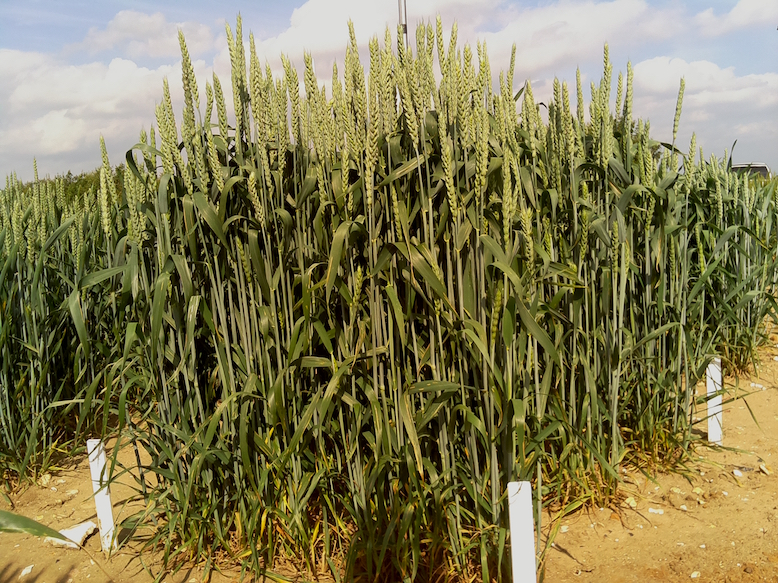
\includegraphics[width=.9\linewidth,height=.7\linewidth,keepaspectratio]{wheat_1.jpg}
  %\caption{MapleTA Question}
  \label{fig:sub1}
\end{subfigure}%
\begin{subfigure}{.5\textwidth}
%  \centering
 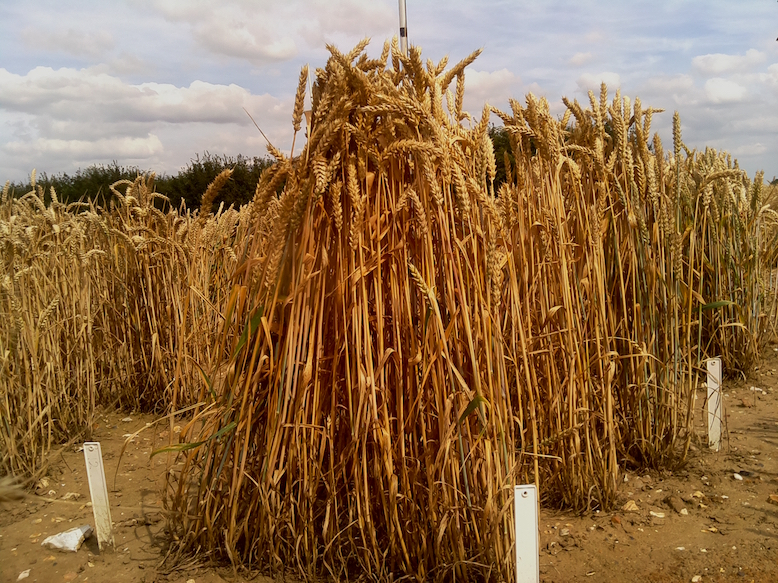
\includegraphics[width=.9\linewidth,height=.7\linewidth,keepaspectratio]{wheat_2.jpg}
  %\caption{MapleTA Gradebook}
  \label{fig:sub2}
\end{subfigure}
\caption{Examples of images from dataset}
\label{fig:test}
\end{figure}
We were provided with 13 high resolution images of a wheat growing plot. The images showed the wheat plants at different stages in their development. The orientation and colour of the wheat stalks different in some of the images. 
The first issue here is that 13 images provides very little data for supervised learning. This makes counting-by-regression approaches unsuitable to this problem. On the other hand, the small size of the dataset made it possible to manually count the grains in each image, essentially providing labels for any approaches that are used with said images as well as targets for evaluation. In the following chapter, we will discuss how the matter of the size of the dataset is dealt with using our proposed approach.






%%% ----------------------------------------------------------------------

